

\section{A Framework: Multiplexing Unentangled States for Property Testing}\label{sec:prop_testing}

In this section, we present a general template illustrating the utility of our disentangler~\cref{thm:channel}. 
We will then use this template multiple of times. Initially, we provide two examples as warm-ups for what is to come. Subsequently, in later sections, we apply this template with carefully designed testers to obtain new complexity results.

Our disentangler leverages a bipartite unentanglement assumption between two states of the form
$\rho_1 \otimes \rho_2$ into an (approximate) multipartite unentanglement assumption of the form $\int \ket\psi\bra\psi^{\otimes k}d\mu$.
Having sufficiently many unentangled copies of a state $\psi$ is particularly important in the context of quantum property
testing as some properties require this assumption for testability. Indeed, many of other information processing
tasks like quantum state tomography often assumes the input is of this form $\ket \psi\bra\psi^{\otimes k}$. Moreover, multiple copies
allow the tester to be executed multiple times amplifying its probability of distinguishing the closeness to
the desired property. Finally, a property tester may end up destroying the copies $\psi^{\otimes k}$ when it measures this state,
so it is desirable to have additional copies that can be used in further information processing tasks once the closeness to
the desired property is certified. In~\cref{fig:dis_and_prop_test}, we provide an illustration of a property
tester being used in conjunction with our disentangler in order to obtain the aforementioned benefits.

\usetikzlibrary{positioning, decorations.pathreplacing, arrows.meta, calc, fit}

\begin{figure}[h]
  \captionsetup{width=.8\linewidth}
  \centering
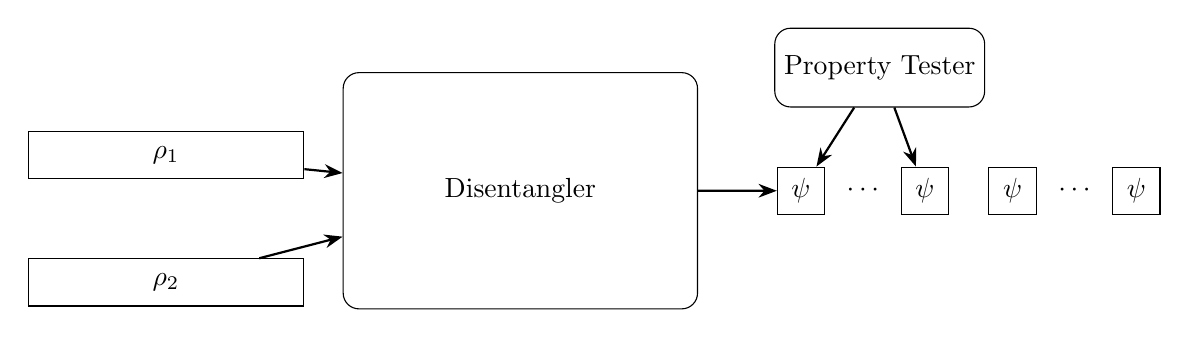
\begin{tikzpicture}[>=Stealth, scale=0.9]

    \tikzstyle{input} = [draw, minimum width=3.5cm, minimum height=0.6cm, align=center]
    \tikzstyle{output} = [draw, minimum width=0.6cm, minimum height=0.6cm, align=center, inner sep=2pt]
    \tikzstyle{operation} = [draw, minimum width=4.5cm, minimum height=3cm, align=center, rounded corners=2mm]
    \tikzstyle{arrow} = [->, thick]
    \tikzstyle{tester} = [draw, minimum width=2cm, minimum height=1cm, align=center, rounded corners=2mm]


    \node[input] (rho1) {$\rho_1$};
    \node[input, below=of rho1] (rho2) {$\rho_2$};
    

    \node[operation] at (5,-0.5) (disentangler) {Disentangler};
    

    \node[output, right=1cm of disentangler] (psi1) {$\psi$};
    \node[right=0.15cm of psi1] (dots1) {$\cdots$};
    \node[output, right=0.15cm of dots1] (psik) {$\psi$};
    
    \node[output, right=0.5cm of psik] (psi1_2) {$\psi$};
    \node[right=0.15cm of psi1_2] (dots2) {$\cdots$};
    \node[output, right=0.15cm of dots2] (psik_2) {$\psi$};
    
    \node[tester, above=0.75cm of psi1, xshift=1cm] (tester) {Property Tester};
    \draw[arrow] (tester) -- (psi1);
    \draw[arrow] (tester) -- (psik);

    \draw[arrow] (rho1) -- (disentangler);
    \draw[arrow] (rho2) -- (disentangler);

    \draw[arrow] (disentangler) -- (psi1);    
\end{tikzpicture}
  \caption{Schematic picture of our disentangler being used to (approximately) ensure multiple unentangled copies of a state as output.
            Part of these copies are used to test a given desired property. If the test passes, the remaining ``certified'' copies can be
            used in further information processing tasks.}\label{fig:dis_and_prop_test}
\end{figure}


\paragraph{Product Tester and Preparing Multipartite Separable States}
To make this illustration more concrete, first we consider a  scenario where the tester is the product test~\cite{HM13}. More precisely, the product test requires two unentangled copies of $\ket{\psi} \in \C^d$ and checks whether
$\ket\psi$ is close to a  product state of the form $\ket{\phi_1}\otimes \cdots \otimes \ket{\phi_s} \in \C^{d_1} \otimes \cdots \otimes \C^{d_s}$,
where $d=d_1\cdots d_s$. 
%This example also shows that even having many copies of the same state in $\int \psi^{\otimes k}d\mu$, the product test can ensure that each $\ket{\psi}$ is itself close to a product state of possibly distinct states of the form $\ket{\phi_1} \otimes \cdots \otimes \ket{\phi_s}$.
For context, %we use the notation $P_{\text{test}}$ from Harrow and Montanaro~\cite{HM13} to refer to the product test and 
recall that (an abridged version of) their main result provides the following guarantees for this tester.

\begin{theorem}[Product Test~\cite{HM13}]\label{theo:prod_test}
  Given $\ket{\psi} \in \C^{d_1} \otimes \cdots \otimes \C^{d_s}$, let
  \[
  1-\epsilon = \max \left\{ \abs{\braket{\psi}{\phi_1,\ldots,\phi_s}}^2 \colon \ket{\phi_i} \in \C^{d_i}, 1 \le i \le s  \right\}\mper
  \]
  Let $P_{\text{test}}(\ket{\psi}\bra{\psi})$ be the probability that the product test passes when applied to $\ket{\psi}$.
  Then, we have $P_{\text{test}}(\ket{\psi}\bra{\psi}) = 1 - \Theta(\epsilon)$.
\end{theorem}

Combining our disentangler from~\cref{thm:channel} and the product test from~\cref{theo:prod_test}, we obtain the
following corollary giving all the desired qualities alluded above in a more quantitative way.

\begin{corollary} \label{cor:separable-states}
  Let $\calH = \C^{d_1} \otimes \cdots \otimes \C^{d_s}$. For every $k,k',\ell \in \N$ such that $\ell\ge k+2k'$, there is a channel $\Gamma \colon \calD( \calH^{\otimes \ell} \otimes \calH^{\otimes \ell}) \to
  \calD(\calH^{\otimes k} \otimes \C^2)$ such that for every $\rho_1,\rho_2 \in \calD( \calH^{\otimes \ell})$, there exists $\sigma \in \calD(\calH^{\otimes k} \otimes \C^2)$
  defined as
  \begin{align*}
    \sigma = \int \ket{\psi}\bra{\psi}^{\otimes k} \otimes \left( P_{\text{test}}(\ket{\psi}\bra{\psi})^{k'}  \ket{1}\bra{1} +  (1-P_{\text{test}}(\ket{\psi}\bra{\psi})^{k'}) \ket{0}\bra{0} \right) d\mu\mcom
  \end{align*}
  such that
  \begin{align*}
    \norm{\Gamma(\rho_1 \otimes \rho_2) -  \sigma}_1 \le \tilde O\left(\left(\frac{(k+2k')^3}{\ell}\right)^{1/4}\right)\mper
  \end{align*}
  Furthermore, $\Gamma(\rho_1 \otimes \rho_2) = (\ket{\psi}\bra{\psi})^{\otimes k} \otimes \ket{1}\bra{1}$ provided
  $\rho_1 = \rho_2 = (\ket{\psi}\bra{\psi})^{\otimes \ell}$, where
  $\ket{\psi} = \ket{\phi_1}\otimes \ldots \otimes \ket{\phi_s}$ for some $\ket{\phi_i} \in \C^{d_i}$ for $1 \le i \le s$.
\end{corollary}  


\begin{proof}
  Define another channel $\Gamma' \colon \calD(\calH^{\otimes( k+2k')}) \to \calD(\calH^{\otimes k} \otimes \C^2)$ that takes as input
  the output of the disentangler $\Lambda$ which is comprised of $k+2k'$ registers of the space $\calH$. 
  We define the channel $\Gamma'$ to act as identity on the first $k$ registers. On the last $2k'$ registers it performs the product test
  on each pair of registers, outputting a single qubit $\ket{1}\bra{1}$ if all tests pass, otherwise outputting $\ket{0}\bra{0}$.
  Next we show $\Gamma = \Gamma' \circ \Lambda$, the composed channel, satisfies the statement.

  Given general input $\rho_1 \otimes \rho_2$, by the guarantee of our disentangler, $\Lambda(\rho_1 \otimes \rho_2)$ satisfies
  \begin{align*}
    \norm{\Lambda(\rho_1 \otimes \rho_2) - \int \ket{\psi}\bra{\psi}^{\otimes k+2k'} d\mu}_1 \le \tilde O\left(\left(\frac{(k+2k')^3}{\ell}\right)^{1/4}\right)\mper
  \end{align*}
  Note that $\Gamma'$ applied to $\int \ket{\psi}\bra{\psi}^{\otimes k+2k'} d\mu$ results in
  \begin{equation}\label{eq:comp_output}
    \int \ket{\psi}\bra{\psi}^{\otimes k} \otimes \left( P_{\text{test}}(\ket{\psi}\bra{\psi})^{k'}  \ket{1}\bra{1} +  (1-P_{\text{test}}(\ket{\psi}\bra{\psi})^{k'}) \ket{0}\bra{0} \right) d\mu \mper
  \end{equation}
  Thus, the composed channel output $\Gamma(\rho_1 \otimes \rho_2))$ is $\tilde O(((k+2k')^3/\ell)^{1/4})$ close, in trace distance, to the state of~(\ref{eq:comp_output}).

  
  The furthermore part is straightforward. Suppose that $\ket{\psi} = \ket{\phi_1}\otimes \ldots \otimes \ket{\phi_s}$, where $\ket{\phi_i} \in \C^{d_i}$ for $1 \le i \le s$,
  and $\rho_1 = \rho_2 = (\ket{\psi}\bra{\psi})^{\otimes \ell}$. In this case, $\Lambda(\rho_1 \otimes \rho_2) = (\ket{\psi}\bra{\psi})^{\otimes k+2k'}$
  and $\Gamma'(\Lambda(\rho_1 \otimes \rho_2)) = (\ket{\psi}\bra{\psi})^{\otimes k} \otimes \ket{1}\bra{1}$ since $\ket{\psi}$ is a product state
  and product test accepts with probability $1$.
\end{proof}

\paragraph{$\QMA(2)$ Tester --- Gap Amplification for $\QMA(2)$}
The gap amplification of $\QMA(2)$ was first proved in the seminar work of Harrow and Montanaro~\cite{HM13}. Using our template, we provide a conceptually more straightforward proof: Take the old $\QMA(2)$ protocol as the property tester in \cref{fig:dis_and_prop_test}.

\begin{theorem}
Given a language $\calL=(\calL_{\mathrm{yes}}, \calL_{\mathrm{no}})$. Suppose that $\calL \in \QMA(2)$ with completeness $c$ and soundness $s$, where $c-s>1/\poly(n)$. Then, $\calL\in\QMA(2)$ with completeness $c'=1-\exp(-\poly(n))$ and soundness $s'=1/\poly(n)$.
\end{theorem}

\begin{proof}
Let $\calP$ be the protocol for $\calL$ with the promised completeness $c$
and soundness $s$. Therefore, for any fixed input $x$ there is a measurement $M$ acting on a space $\calH^{\otimes 2}$ where $\calH=\C^{d}$, such that,
\begin{align}
        &\exists \sigma\otimes \rho \in \calD(\calH^{\otimes 2}), \; 
            \trace(M (\sigma\otimes\rho) ) \ge c,
                &\text{if } x\in \calL_{\mathrm{yes}}
        \nonumber \\
        &\forall \sigma\otimes\rho \in \calD(\calH^{\otimes 2}), \; 
            \trace(M (\sigma\otimes\rho) ) \le s,
                &\text{if } x\in \calL_{\mathrm{no}.}
        \nonumber
\end{align}
In the new protocol, choose $k=\poly(n)/(c-s)^2$ and $\ell=\poly(k)$ for some large enough polynomial. We ask for two proofs $\ket{\rho_1}, \ket{\rho_2} \in \calD(\calH'^{\otimes\ell}),$ where $\calH'=\C^2 \otimes \calH$. In words, $\calH'$ is $\calH$ with one extra qubit. Apply the disentangler $\Lambda$ from~\cref{thm:channel} on $\rho_1\otimes\rho_2$, obtaining a separable state $\phi=\int d\mu \ket\psi\bra\psi ^{\otimes k}$, such that
\begin{equation}
    \left\|\Lambda(\rho_1\otimes\rho_2)-\int d\mu \ket\psi\bra\psi ^{\otimes k}\right\|_1 = \frac{1}{\poly(n)}.\label{eq:gap-amp-error}
\end{equation}
Consider the new measurement $M'=|01\rangle\langle01|\otimes M$. We apply $M'^{\otimes (k/2)}$ to $\Lambda(\rho_1\otimes\rho_2)$. Accept if more than $(c+s)/2$ fraction of the applications of $M'$ accepts; reject otherwise. Next, we calculate the completeness and soundness of the new protocol.

\emph{Completeness.} Suppose that $x\in\calL_{\mathrm{yes}}$, then the faithful prover will provide
\[
    \ket{\rho_1}=\ket{\rho_2}=\left(\frac{|0,\sigma\rangle+|1,\rho\rangle}{\sqrt{2}}\right)^{\otimes \ell}, \text{ and } \Lambda(\rho_1\otimes\rho_2)=\left(\frac{|0,\sigma\rangle+|1,\rho\rangle}{\sqrt{2}}\right)^{\otimes k}.
\]
Calculating the probability that $M'$ accepts $(|0,\sigma\rangle+|1,\rho\rangle)^{\otimes 2}/2$,
\[
    \trace\left( M' \left(\frac{|0,\sigma\rangle+|1,\rho\rangle}{\sqrt2}\right)^{\otimes 2}
    \right) = \frac{1}{4}\trace( M (\sigma\otimes \rho))\ge c/4.
\]
By Chernoff bound, with probability at least $1-\exp(-\Omega((c-s)^2 k))=1-\exp(-\poly(n))$, the new protocol accepts.

\emph{Soundness.} Suppose that $x\in\calL_{\mathrm{no}}$. 
Calculating the probability that $M'$ accepts $(\alpha|0,\sigma\rangle+\beta|1,\rho\rangle)^{\otimes 2}$ for arbitrary $\alpha,\beta \in \C$ and arbitrary $\sigma, \rho\in \calH$ such that $|\alpha|^2+|\beta|^2=1$,
\[
    \trace( M' (\alpha|0,\sigma\rangle+\beta|1,\rho\rangle)^{\otimes 2}
     =|\alpha\beta|^2\trace( M (\sigma\otimes \rho))\le s/4.
\]
Therefore the probability to accept $\phi$, an arbitrary convex combination of $\ket\psi^{\otimes k}$ is at most $\exp(-\Omega((c-s)^2 k))$ by Chernoff bound. Finally, by (\ref{eq:gap-amp-error}), the probability of accepting $\Lambda(\rho_1\otimes\rho_2)$ is at most $1/\poly(n).$
\end{proof}

